\section{Chuyển sang lược đồ quan hệ}

Từ mô hình quan niệm, các thực thể được chuyển thành quan hệ. Mỗi quan hệ có khóa chính để định danh dòng; khóa ngoại biểu diễn liên kết giữa các quan hệ. Các quan hệ $1:N$ được chuyển bằng khóa ngoại ở phía $N$, còn quan hệ $M:N$ được tách thành quan hệ liên kết.

\section{Lược đồ quan hệ đề xuất}

Để lược đồ quan hệ dễ đọc và dễ đối chiếu với các yêu cầu nghiệp vụ, các bảng được nhóm theo bốn miền: \textit{Master Data}, \textit{Inventory}, \textit{Sales} và \textit{Purchasing/Transfer}. Trong đó, \texttt{PRODUCT\_VARIANT/SKU} được đặt làm đơn vị trung tâm vì SKU là đơn vị được bán, định giá, giữ hàng và quản lý tồn kho.

\begin{figure}[H]
    \centering
    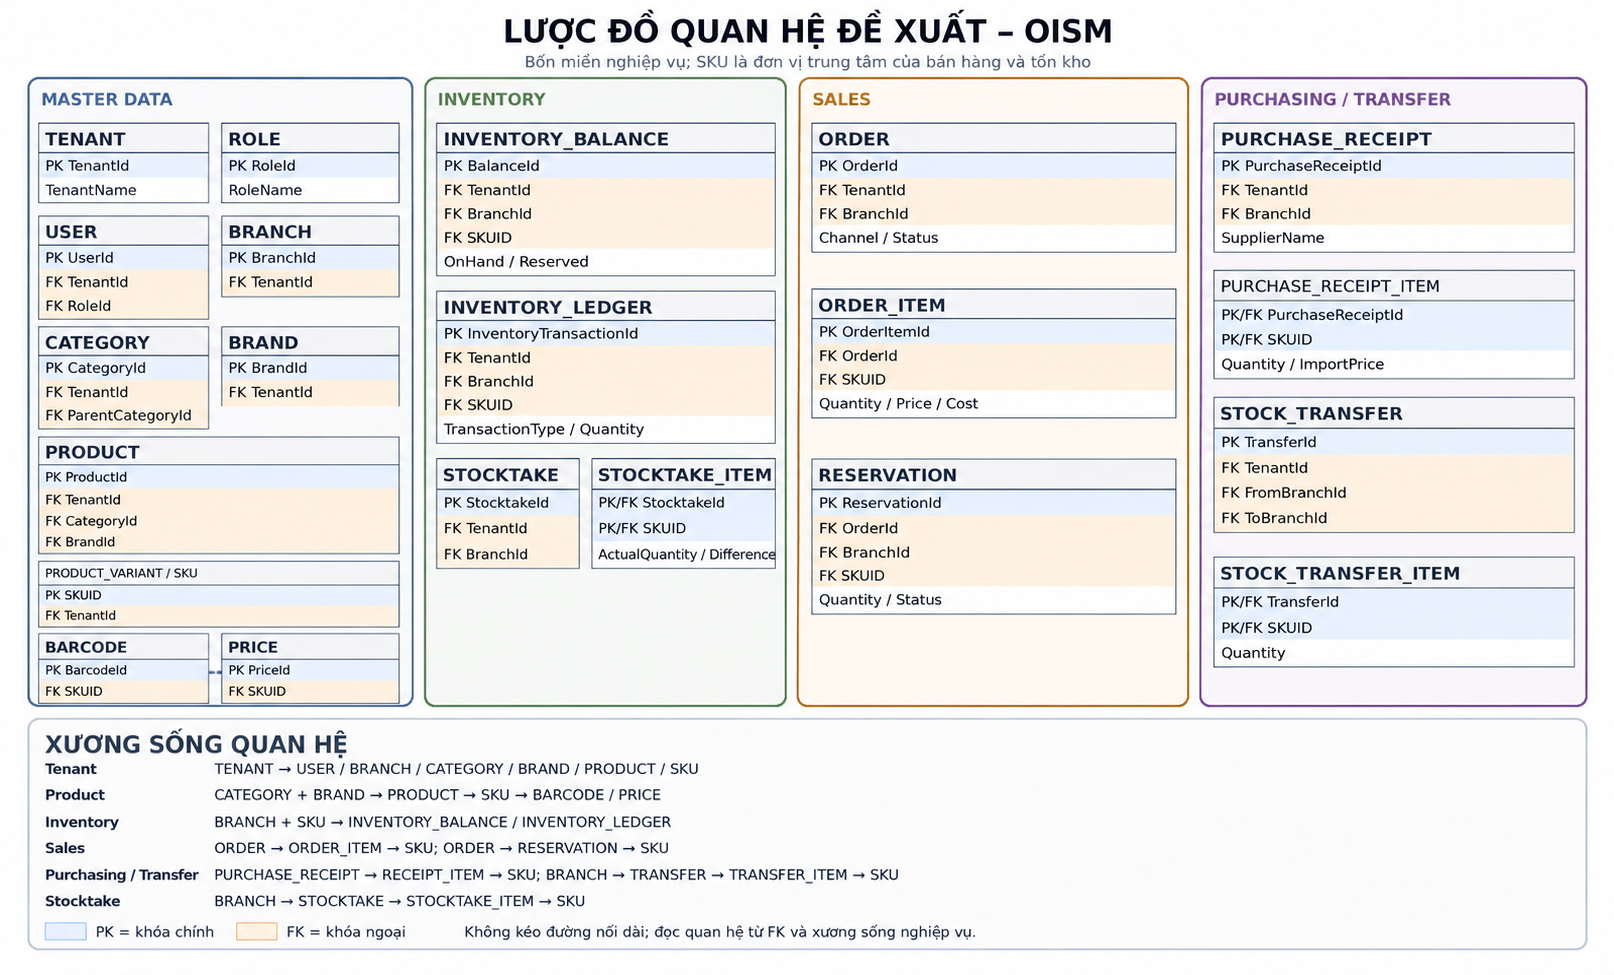
\includegraphics[width=\textwidth,keepaspectratio]{figures/LDQH.png}
    \caption{Lược đồ quan hệ đề xuất theo nhóm nghiệp vụ}
    \label{fig:logical-schema-oism}
\end{figure}

Hình \ref{fig:logical-schema-oism} sử dụng các hộp quan hệ thay vì ký hiệu hình thoi của ERD. PK được đánh dấu màu xanh nhạt, FK được đánh dấu màu cam nhạt. Các quan hệ được đọc trực tiếp từ FK và phần ``xương sống quan hệ'' ở cuối hình, do đó không cần kéo nhiều đường nối dài giữa các miền và tránh tình trạng đường giao nhau hoặc chồng chéo.

\subsection{Danh mục quan hệ}

\begin{description}
    \item[Master Data:] \texttt{TENANT}, \texttt{ROLE}, \texttt{USER}, \texttt{BRANCH}, \texttt{CATEGORY}, \texttt{BRAND}, \texttt{PRODUCT}, \texttt{PRODUCT\_VARIANT/SKU}, \texttt{BARCODE}, \texttt{PRICE}.
    \item[Inventory:] \texttt{INVENTORY\_BALANCE}, \texttt{INVENTORY\_LEDGER}, \texttt{STOCKTAKE}, \texttt{STOCKTAKE\_ITEM}.
    \item[Sales:] \texttt{ORDER}, \texttt{ORDER\_ITEM}, \texttt{RESERVATION}.
    \item[Purchasing/Transfer:] \texttt{PURCHASE\_RECEIPT}, \texttt{PURCHASE\_RECEIPT\_ITEM}, \texttt{STOCK\_TRANSFER}, \texttt{STOCK\_TRANSFER\_ITEM}.
\end{description}

Các quan hệ chính và thuộc tính quan trọng được thống nhất như sau:

\begin{verbatim}
TENANT(TenantId PK, TenantName, CreatedAt)
ROLE(RoleId PK, RoleName)
USER(UserId PK, TenantId FK, RoleId FK, Email, Phone, PasswordHash, CreatedAt)
BRANCH(BranchId PK, TenantId FK, BranchName, Address, IsActive)
CATEGORY(CategoryId PK, TenantId FK, ParentCategoryId FK NULL, CategoryName)
BRAND(BrandId PK, TenantId FK, BrandName)
PRODUCT(ProductId PK, TenantId FK, CategoryId FK, BrandId FK,
        ProductName, Description)
PRODUCT_VARIANT(SKUId PK, TenantId FK, ProductId FK, SKUCode,
                VariantName, ReorderThreshold)
BARCODE(BarcodeId PK, TenantId FK, SKUId FK, BarcodeValue, BarcodeType)
PRICE(PriceId PK, TenantId FK, SKUId FK, RetailPrice, WholesalePrice,
      EffectiveFrom, EffectiveTo)
INVENTORY_BALANCE(BalanceId PK, TenantId FK, BranchId FK, SKUId FK,
                  OnHand, Reserved, VersionNo)
INVENTORY_LEDGER(InventoryTransactionId PK, TenantId FK, BranchId FK,
                 SKUId FK, TransactionType, Quantity, BalanceAfter,
                 ReferenceId, CreatedAt)
PURCHASE_RECEIPT(PurchaseReceiptId PK, TenantId FK, BranchId FK,
                 SupplierName, ReceiptDate, Status)
PURCHASE_RECEIPT_ITEM(PurchaseReceiptId PK/FK, SKUId PK/FK,
                      Quantity, ImportPrice)
ORDER(OrderId PK, TenantId FK, BranchId FK, Channel, Status,
      OrderDate, CustomerReference)
ORDER_ITEM(OrderItemId PK, OrderId FK, SKUId FK, Quantity,
           SellingPrice, CostPrice)
RESERVATION(ReservationId PK, TenantId FK, OrderId FK, BranchId FK,
            SKUId FK, Quantity, Status, CreatedAt, ReleasedAt)
STOCK_TRANSFER(TransferId PK, TenantId FK, FromBranchId FK,
               ToBranchId FK, Status, CreatedAt, ConfirmedAt)
STOCK_TRANSFER_ITEM(TransferId PK/FK, SKUId PK/FK, Quantity)
STOCKTAKE(StocktakeId PK, TenantId FK, BranchId FK, StocktakeDate, Status)
STOCKTAKE_ITEM(StocktakeId PK/FK, SKUId PK/FK,
               SystemQuantity, ActualQuantity, Difference)
\end{verbatim}

\section{Giải thích một số quan hệ quan trọng}

\subsection{INVENTORY\_LEDGER và INVENTORY\_BALANCE}

\texttt{INVENTORY\_LEDGER} là lịch sử biến động và có tính chất append-only. \texttt{INVENTORY\_BALANCE} là trạng thái hiện tại được duy trì để đọc nhanh. Hai bảng không có cùng vai trò: Balance không thay thế Ledger. Khi số dư thay đổi, cập nhật Balance và ghi Ledger phải nằm trong cùng giao dịch để tránh hai nguồn dữ liệu tách rời.

\subsection{ORDER và ORDER\_ITEM}

ORDER lưu thông tin chung của đơn; ORDER\_ITEM lưu các SKU cụ thể. \texttt{CostPrice} trong ORDER\_ITEM là giá vốn snapshot tại thời điểm hoàn tất, giúp báo cáo COGS lịch sử không bị thay đổi bởi WAC tương lai.

\subsection{RESERVATION}

RESERVATION lưu lượng hàng đang được giữ cho đơn. Số lượng có thể bán được tính từ số dư hiện tại:
\[
Available = OnHand - Reserved.
\]

\section{Khóa và ràng buộc}

Các khóa chính phải NOT NULL và duy nhất. Khóa ngoại phải tham chiếu đến bản ghi tồn tại. Các thuộc tính như SKUCode, BarcodeValue có thể cần UNIQUE trong phạm vi tenant. Số lượng hàng phải không âm ở những trường phù hợp; giá tiền không âm; trạng thái phải thuộc tập giá trị được định nghĩa.

Đối với quan hệ theo tenant, các thao tác truy vấn phải kiểm tra TenantId. Ràng buộc này là một phần của thiết kế toàn vẹn dữ liệu, không chỉ là quy tắc giao diện.
